\documentclass[dvipdfmx]{jsarticle}
%
\usepackage{amsmath}
\usepackage{emath}
\usepackage[dvipdfmx]{graphicx}
\usepackage{mediabb}%pdfを簡単に取り込み
\usepackage{here}
\usepackage{ascmac}%screenのため
\usepackage{yhmath}%長いtildeのため
\usepackage{color}
\usepackage{ulem}%取り消し線のため
\allowdisplaybreaks[4]%式変形中の改ページの許可
\usepackage[dvipdfmx]{hyperref}%ハイパーリンクの埋め込み
\usepackage{pxjahyper} %%hyperref読み込みの直後に読み込んでおくおまじない
\usepackage[all]{xy}%xypic
\usepackage{comment}
%
\pagestyle{plain}
\title{黒田関数解析}
\author{\empty}
\date{\today}
%
\newtheorem{definition}{定義}[section]%section単位でカウントをリセット
\newtheorem{instance}{例}[section]%定義から通し番号にする
\newtheorem{theorem}{定理}[section]%section単位でカウントをリセット.こうしておくとsetcounterで番号をコントロールできる
\newtheorem{prop}{命題}[section]
\newtheorem{lemma}{補題}[section]
\newtheorem{corollary}{系}[section]
\newtheorem{example}{例題}[section]
\makeatletter
\def\th@plain{\upshape}%定理環境で斜体を使わないためのおまじない
\makeatother
%
%\newtheorem{definition}{定義}[section]%section単位でカウントをリセット
%\newtheorem{instance}[definition]{例}%定義から通し番号にする
%\newtheorem{theorem}[definition]{定理}
%\newtheorem{prop}[definition]{命題}
%\newtheorem{lemma}[definition]{補題}
%\newtheorem{corollary}[definition]{系}
%\makeatletter
%\def\th@plain{\upshape}%定理環境で斜体を使わないためのおまじない
%\makeatother
%
\newtheorem{proof}{証明}
\renewcommand{\theproof}{}%カウントしない
\usepackage{latexsym}
\def\qed{\hfill $\Box$}
%
\newtheorem{agree}{規約}
\renewcommand{\theagree}{}%カウントしない
\newtheorem{attention}{注意}
\renewcommand{\theattention}{}%カウントしない
%
\newcommand{\st}{\mathrm{s.t.}\,}  %s.t.
%
%おまじない
\setlength{\textwidth}{\fullwidth}
\setlength{\textheight}{39\baselineskip}
\addtolength{\textheight}{\topskip}
\setlength{\voffset}{-0.5in}
\setlength{\headsep}{0.3in}
\setlength{\abovedisplayskip}{3pt}%上部のマージン
\setlength{\belowdisplayskip}{3pt}%下部のマージン
%
%一応引き継いで書いてあるが,今は機能していない
\usepackage{stmaryrd}%\longmapsfrom
\usepackage{bm}%数式中の太字
\usepackage{graphicx}%写像の図式のため
\usepackage[all]{xy}%xypic
%
\begin{document}
%\maketitle
%
\begin{itembox}[l]{定理7.21(一様有界性原理)}
$\mathcal{X}$をBanach空間,$\mathcal{Y}$をノルム空間であるとし,$\{T_\lambda\}_{\lambda\in\Lambda}$を$B(\mathcal{X},\mathcal{Y})$に属する族とする.このとき
\begin{align*}
^\forall u\in\mathcal{X},{\ }\sup_{\lambda\in\Lambda}{||T_\lambda u||}<\infty {\ }\Longrightarrow{\ } \sup_{\lambda\in\Lambda}{||T_\lambda||}<\infty
\end{align*}
となる.言い換えれば,$\mathcal{X}$の各点$u$で$\{T_\lambda u\}_{\lambda\in\Lambda}$が有界ならば,$\{T_\lambda\}_{\lambda\in\Lambda}$は一様に有界である.
\end{itembox}
\vspace{-0.7zh}%間隔調整
\vspace{-0.7zh}%間隔調整
\vspace{-0.7zh}%間隔調整
\begin{proof}
{\ }
\begin{figure}[H]
\begin{center}
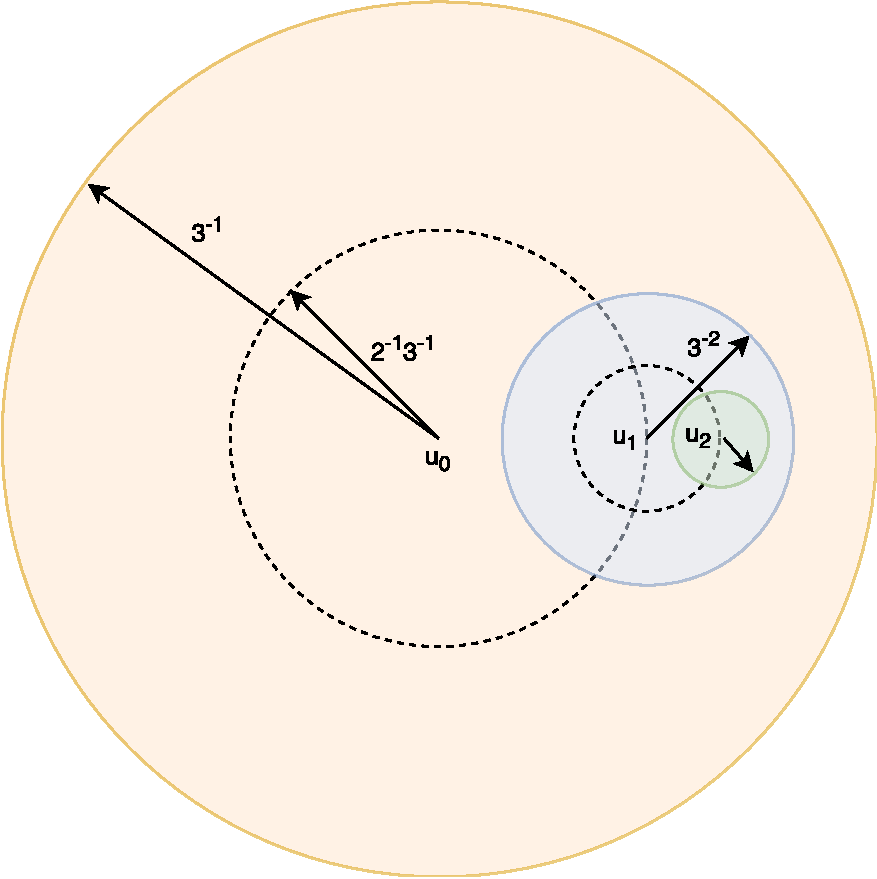
\includegraphics[width=0.6\textwidth]{ubp-fig.pdf}
\label{baire}
\end{center}
\end{figure}
%
\cite{Sokal}による初等的で簡潔な証明を紹介する.まず,簡単な補題を示す.$T\in B(\mathcal{X},\mathcal{Y})$とする.中心$u$半径$r$の閉球を$\mathcal{C}(u,r)$と書く.$^\forall u\in\mathcal{X}$を固定すれば
\begin{align*}
\max\{||T(u+u')||,||T(u-u')||\}\geq\frac{1}{2}\left(||T(u+u')||+||T(u-u')||\right)\geq ||Tu'|| \quad ( ^\forall u'\in\mathcal{X})
\end{align*}
となる.ただし,最後の不等号においては三角不等式を用いた.$^\forall r>0$に対して,$u'\in \mathcal{C}(0,r)$について左辺から右辺の順に$\sup$を取れば
\begin{align*}
\sup_{u''\in \mathcal{C}(u,r)}||Tu''||\geq \sup_{u'\in \mathcal{C}(0,r)}||Tu'||=\sup_{u'\in \mathcal{C}(0,1)}||Tu'||r=||T||r
\end{align*}
となるので,左辺で$u''\to u'$と文字を取り換えれば
\begin{equation*}
\sup_{u'\in \mathcal{C}(u,r)}||Tu'||\geq ||T||r \eqno(\ast)
\end{equation*}
が成り立つ.\par
以下が証明の本筋である.$\underset{\lambda\in\Lambda}{\sup}{||T_\lambda||}=\infty$と仮定して対偶を示す.$\underset{\lambda\in\Lambda}{\sup}{||T_\lambda||}=\infty$より,$\{T_n\}_{n=1}^\infty$を$||T_n||\geq 4^n$となるように取ることができる.一方,$u_0:=0\in\mathcal{X}$とすると,$(\ast)$で$u=u_0,{\ }r=2^{-1}3^{-1},{\ }T=T_1$として
\begin{align*}
^\exists u_1\in\mathcal{C}(u_0,2^{-1}3^{-1}) \Longrightarrow ||u_1-u_0||\leq 2^{-1}3^{-1},{\ }||T_1 u_1||\geq 2^{-1}3^{-1}||T_1||
\end{align*}
が成り立つので,特に
\begin{align*}
\mathcal{C}(u_1,3^{-2})\subset\mathcal{C}(u_0,3^{-1}),\quad ||u_1-u_0||<3^{-1},\quad ||T_1 u_1||\geq 2^{-1}3^{-1}||T_1||
\end{align*}
が成り立つ.同様に,$(\ast)$で$u=u_1,{\ }r=2^{-1}3^{-2},{\ }T=T_2$として
\begin{align*}
^\exists u_2\in\mathcal{C}(u_1,2^{-1}3^{-2})\subset \mathcal{C}(u_0,2^{-1}3^{-2}) \Longrightarrow ||u_2-u_1||\leq 2^{-1}3^{-2},{\ }||T_2 u_2||\geq 2^{-1}3^{-2}||T_2||
\end{align*}
が成り立つので,特に
\begin{align*}
\mathcal{C}(u_2,3^{-3})\subset\mathcal{C}(u_1,3^{-2})\subset\mathcal{C}(u_0,3^{-1}),\quad ||u_2-u_1||<3^{-2},\quad ||T_2 u_2||\geq 2^{-1}3^{-2}||T_2||
\end{align*}
が成り立つ.帰納的に,$u_k\in\mathcal{X}{\ }(n=0,1,2,\cdots)$を
\begin{equation*}
\mathcal{C}(u_n,3^{-(n+1)})\supset\mathcal{C}(u_{n+1},3^{-(n+2)})\supset\cdots \quad (n=0,1,2,\cdots)
\end{equation*}
\begin{equation*}
||u_n-u_{n-1}||<3^{-n},\quad ||T_n u_n||\geq 2^{-1}3^{-n}||T_n|| \quad (n=1,2,\cdots)
\end{equation*}
を満たすように取ることができる.$\{u_n\}_{n=0}^{\infty}$はコーシー列であるので,$\mathcal{X}$が完備であることから$^\exists u\in\mathcal{X}$に収束する.ここで,$^\forall m=0,1,2,\cdots$に対して$n=m$として固定すると,$^\forall n\geq m$に対して$u_n\in \mathcal{C}(u_m,2^{-1}3^{-(m+1)})$であるので,$u\in \mathcal{C}(u_m,2^{-1}3^{-(m+1)})$となる.$m$は$^\forall m=0,1,2,\cdots$に対して成り立つので,特に
\begin{align*}
||u-u_n||<3^{-(n+1)} \quad (n=0,1,2,\cdots)
\end{align*}
が成り立つ.よって,ノルムの定義より
\begin{align*}
||T_n u-T_n u_n||\leq ||T_n||\cdot||u-u_n||<3^{-(n+1)}||T_n|| \quad (n=1,2,\cdots)
\end{align*}
となるので,上で得られた等式と不等式より
\begin{align*}
||T_n u||\geq ||T_n u_n||-||T_n u-T_n u_n||>6^{-1}3^{-n}||T_n||\geq 6^{-1}\left(\frac{4}{3}\right)^n\to\infty \quad (n\to\infty)
\end{align*}
が成り立つ.よって,対偶が示された.
\qed
\end{proof}
%
%
%
\begin{thebibliography}{99}
\bibitem{kuroda}
  黒田成俊『共立数学講座15 関数解析』(共立出版,1980年)
\bibitem{Sokal}
  Alan D. Sokal, “A really simple elementary proof of the uniform boundedness theorem”
  \href{https://arxiv.org/abs/1005.1585}{arXiv:1005.1585v2 [math.FA]}
\end{thebibliography}
%
%
%
%
\end{document}